\clearpage
\section{Experiments}

\subsection{First implementation}
\begin{itemize}
\item Do some experiments to see that you can create a group, add some peers and keep their state coordinated. 
\begin{figure}[h!]
\centering
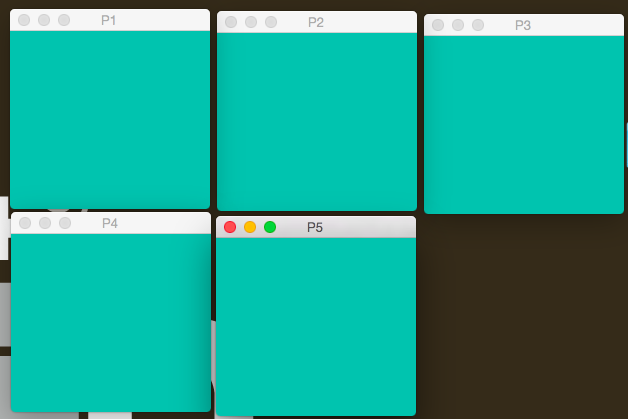
\includegraphics[scale=0.7]{resources/img/exp1.png}
\caption{Module gms1, sleep 2000}
\end{figure}
\newline\textit{In the experiements we can see that the different nodes do synchronized state changes. This is due to the total ordering of the multicast layer. There are no crashes in this module, so the nodes don't get out of sync.}


\clearpage
\item Split the groupy module and make the needed
adaptations to enable each worker to run in diferent machines. Remember
how names registered in remote nodes are referred and how Erlang runtime
should be started to run distributed programs.
\inputminted[
    fontsize=\small,
    linenos,
    firstline=11,
    lastline=38]{erlang}{resources/src/groupy.erl}
\end{itemize}
\textit{We achieved this by spawning processes, similiar to ordy the program.}

\clearpage
\subsection{Failure detectors}
\begin{itemize}
\item Do some experiments to see if the peers can keep their state coordinated even if nodes crash.

x

\end{itemize}, 
\newline\textit{Yes, normally the nodes keep their coordinated state , even if the leader crashes. This is due to the fact that the nodes only get out of sync if the leader crashes during a multicast. Then it might happen that only a some of the nodes receive the message that the leader was sending. As a consecuence the nodes are out of sync from this moment on.}

\clearpage
\subsection{Missing Messages}
\begin{itemize}
\item Repeat the experiments and see if you can have the state
of the workers come out of sync.
\begin{figure}[h!]
\centering
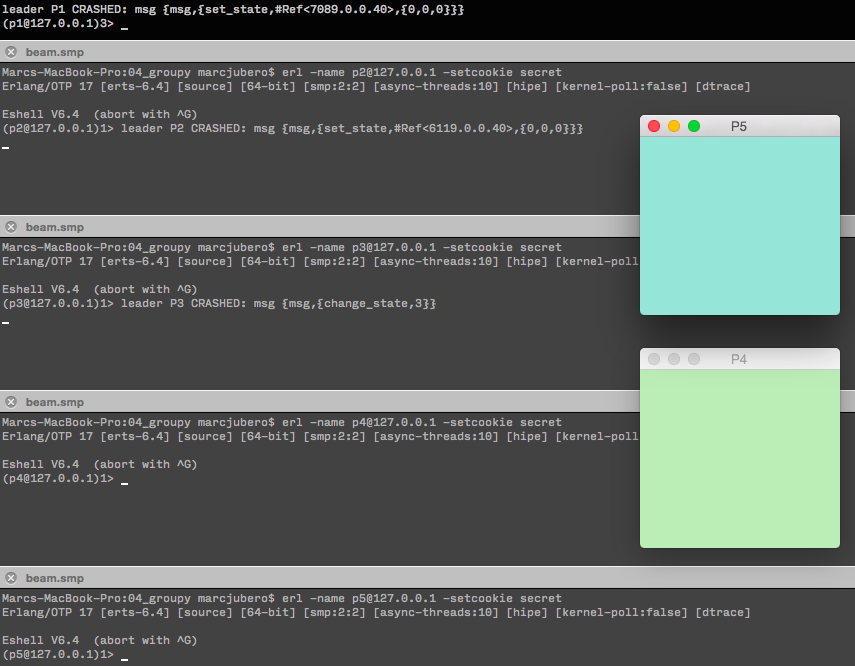
\includegraphics[scale=0.4]{resources/img/exp3.png}
\caption{Module gms2, sleep 2000}
\end{figure}
\newline\textit{It is possible, as we stated before, that the workers come out of sync, if the leader crashes during a multicast because only some of the client nodes will receive the message that is multicasted. So we achieved this by implementing crashes with certain probability that happen during the multicast. As a consecuence, we can see how the workers get out of sync.}

\end{itemize}

\subsection{Reliable Multicast}
\begin{itemize}
\item Repeat the experiments to see if now the peers can keep their state coordinated even if nodes crash.
\newline\textit{Yes, they can because we implemented a reliable multicast in the gsm3 module. A reliable multicast keeps track of the messages by using secuence numbers. Every slave that receives a message compares its secuence number to the secuence number of the last one that is has delivered. If the incoming message has the the expected secuence number, if it is smaller, it will be discarded.}
\newline\textit{If a slave becomes the new leader it resends the last message it has received from the leader. That is why every slave always stores the last received message. As the leader always sends the messages in the order as the nodes appear in the view list and the new leader in case of crash will be the first in this list, if somebody has reveived the last message of the leader, it will be the new leader.}
\newline\textit{That is how reliable multicast is implemented.}
\end{itemize}

